\section{\label{I-B-1}Un musée d'exception sous contraintes : une dépendance étroite du \minarm}

Bien qu'il soit reconnu comme un musée de France au patrimoine exceptionnel, le \mae ne jouit pas d'une véritable autonomie. Placé dès sa naissance sous la tutelle du sous-secrétaire d'État à l'aéronautique militaire et maritime\footcite{terrierAeroportParisBourget2019}, il suit les évolutions institutionnelles de celui-ci : ministère de l'Air en 1928, rattachement au ministère de la Défense nationale en 1948, puis changements successifs de dénomination. Aujourd'hui sous l'autorité du \minarm, il est rattaché à la \gls{dmca}.

Juridiquement, cette tutelle se traduit par le statut d'« établissement public national à caractère administratif doté de la personnalité civile et de l'autonomie financière » que lui confère l'article R3413-1 du Code de la défense\footcite{ArticleR34131Code2008}. Ce statut, défini par le décret n°2008-1219 du 25 novembre 2008, place formellement le musée sous la tutelle du ministre de la Défense (aujourd'hui ministre des Armées) et lui assigne pour mission d'« assurer la conservation et l'enrichissement des collections de l'État ainsi que la présentation au public du patrimoine historique et culturel national dans le domaine de l'aéronautique et de l'espace ». Son organisation administrative reflète ce statut : le conseil d'administration comprend notamment un membre du Conseil d'État, douze représentants des administrations de l'État — dont les chefs d'état-major des trois armées — et huit personnalités choisies par le ministre de la Défense\footcite{ArticleR341373Code2013}. Le directeur est nommé par arrêté du ministre de la Défense.

Le réseau institutionnel\footnote{Voir la carte \refinterne{fig:cart_musees}} dans lequel s'inscrit le \mae est défini par une instruction ministérielle du 20 mars 2023\footcite{ministeredesarmeesInstructionNdeg303ARM2023}.
Celle-ci distingue plusieurs catégories d'établissements culturels militaires : le \mae fait partie des sept musées du \minarm à bénéficier de l'appellation \enquote{musée de France} depuis 2002. Ce statut le distingue notamment \enquote{musées de tradition}, \enquote{conservatoires}, ou des \enquote{centres d'interprétation} qui ne disposent pas de la même protection juridique. Ce réseau, très diversifié, comprend par exemple de grands musées parisiens comme le musée de l'armée aux Invalides ou le musée de la Marine, ainsi que et ses 4 antennes en région, des institutions qui bénéficient d'un prestige moindre comme le musée du Service de Santé des Armées au Val de Grâce, celui du Génie à Angers, ou des bien plus petites comme celle du Mémorial du Débarquement et de la Libération en Provence à Toulon.
\footnote{Voir \url{https://www.defense.gouv.fr/sga/memoire-culture-archives/culture/musees}}.


\begin{figure}[htbp]
	\centering
	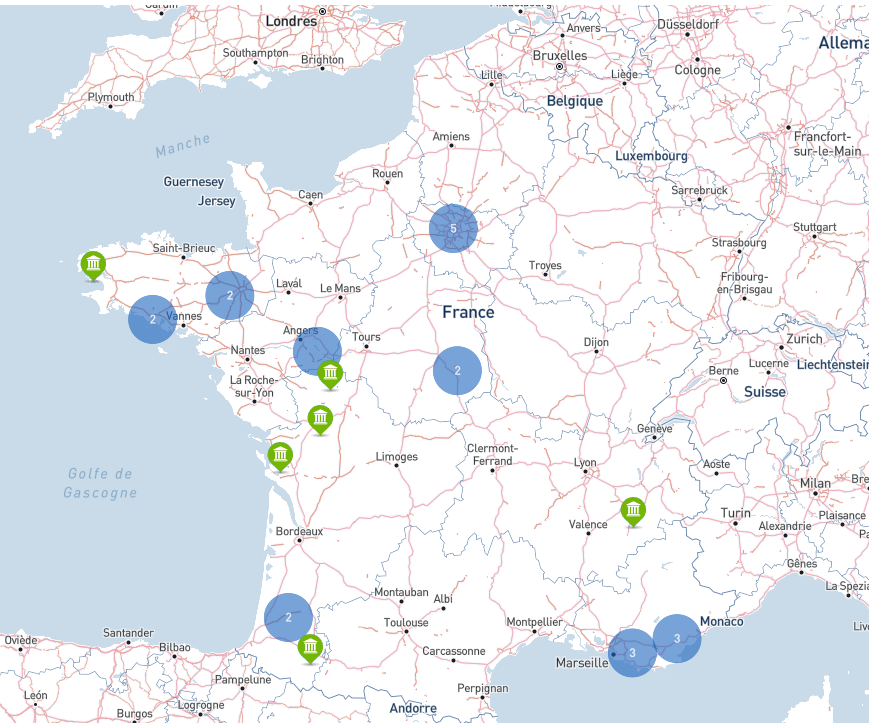
\includegraphics[width=\linewidth]{img/CART_musees_armee}
	\caption[Cartographie du réseau des musées du \minarm]{De nombreux musées dépendent aujourd'hui du \minarm~(carte disponible sur \href{https://www.memoiredeshommes.sga.defense.gouv.fr/musees-collections-et-mecenat/musees-et-monuments}{Mémoire des hommes}).}
	\label{fig:cart_musees}
\end{figure}


Tant du point de vue financier que culturel, le \mae dépend de politiques générales aux musées du ministère de l'Armée puisqu'il a une fonction de représentation de sa mémoire\footcite{museedelairetdelespaceProjetScientifiqueCulturel2020}. Il est donc pris dans un faisceau de décisions qui conditionnent ses évolutions techniques, documentaires ou institutionnelles : ainsi, jusqu'aux années 2000, agents et directeurs du musée étaient en grande partie issus du milieu militaire. Cette particularité de l'institution a pu contribuer à la création d'un décalage dans l'évolution de l'institution  par rapport à celle d'autres dont les agents seraient issus des professionnels des musées. Cette impression généralisée au \ac{dsc} provient également du décalage inverse qui existe aujourd'hui, lorsque l'intégralité des agents du musée -- mis à part un officier de liaison -- sont issus du monde civil et ne partagent pas toujours la même culture que l'institution publique qu'ils représentent.

Cette intégration dans un vaste réseau d'institution dont les profils, les besoins et les missions peuvent être très différents aura donc un impact important sur le quotidien du musée : ceci se traduit par exemple dans la complexité des procédures qui peuvent être nécessaires pour mettre en place de nouveaux projets lorsqu'ils nécessitent des fonds ou une mise en place particulière. En effet, certains choix ne concerneront pas uniquement le \mae et toucheront également l'ensemble des musées du réseau.
